\section{Modular Coding and Linking}

\begin{concept}{Modular Programming Overview}\\
Program code is divided into modules with:
\begin{itemize}
  \item Each source file compiled into separate object file
  \item All object files linked into single executable
  \item Clear interfaces between modules
\end{itemize}

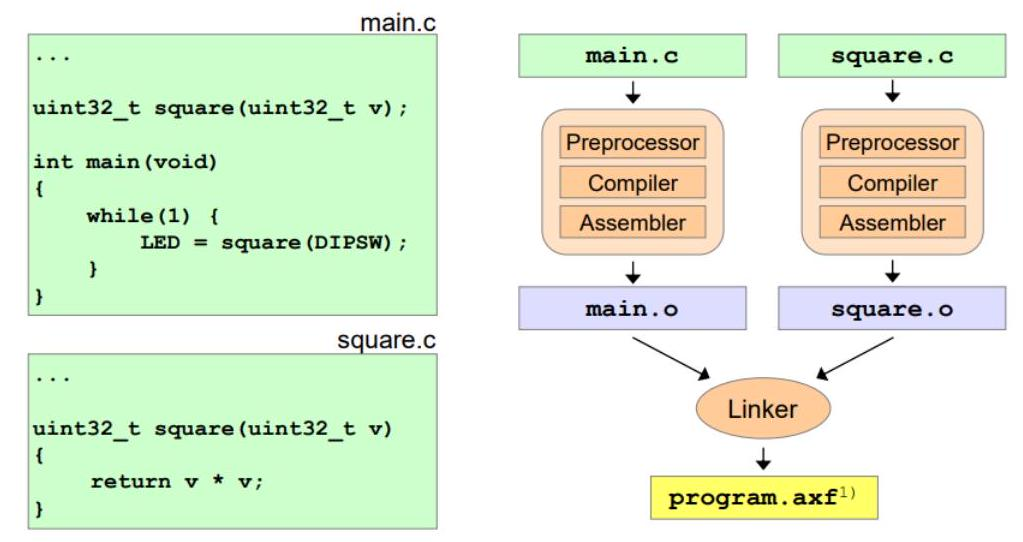
\includegraphics[width=\linewidth]{images/2024_12_29_79e6b22f503fb7b4f718g-10(2)}
\end{concept}

\begin{definition}{Benefits of Modular Programming}\\
Key advantages:
\begin{itemize}
  \item \textbf{Team Development}:
    \begin{itemize}
      \item Multiple developers working on same codebase
      \item Clear ownership of modules
    \end{itemize}
  \item \textbf{Code Organization}:
    \begin{itemize}
      \item Logical partitioning of functionality
      \item Easier code reuse
    \end{itemize}
  \item \textbf{Development Efficiency}:
    \begin{itemize}
      \item Individual module testing
      \item Faster compilation (only changed modules)
      \item Reusable library creation
    \end{itemize}
  \item \textbf{Language Integration}:
    \begin{itemize}
      \item Mix C and assembly modules
      \item Language-specific optimizations
    \end{itemize}
\end{itemize}
\end{definition}

\begin{definition}{Module Linkage}\\
Keywords for controlling module interfaces:
\begin{itemize}
  \item \textbf{EXPORT}: Make symbol available to other modules
  \item \textbf{IMPORT}: Use symbol from another module
  \item Internal symbols: Neither IMPORT nor EXPORT
\end{itemize}

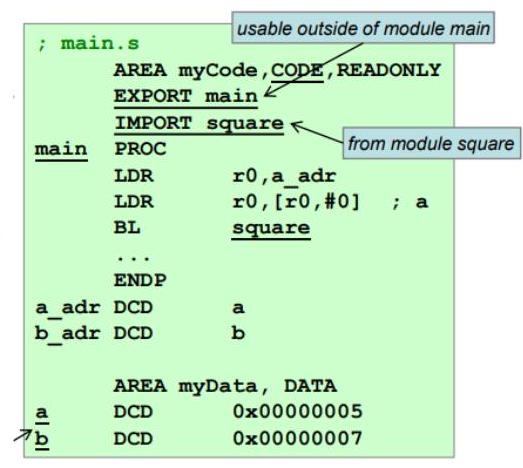
\includegraphics[width=\linewidth]{images/2024_12_29_79e6b22f503fb7b4f718g-10(1)}
\end{definition}

\begin{definition}{Object Files}\\
ELF format contains:
\begin{itemize}
  \item \textbf{Code Section}:
    \begin{itemize}
      \item Program code and constants
      \item Based at address 0x0
    \end{itemize}
  \item \textbf{Data Section}:
    \begin{itemize}
      \item Global variables
      \item Based at address 0x0
    \end{itemize}
  \item \textbf{Symbol Table}:
    \begin{itemize}
      \item All symbols and their attributes
      \item Global/local status
      \item References to external symbols
    \end{itemize}
  \item \textbf{Relocation Table}:
    \begin{itemize}
      \item Instructions for adjusting addresses
      \item Applied during linking process
    \end{itemize}
\end{itemize}
\end{definition}

\begin{concept}{Linker Operation}\\
Main tasks:
\begin{itemize}
  \item Merge code sections from all objects
  \item Merge data sections from all objects
  \item Resolve symbol references between modules
  \item Relocate addresses to final positions
\end{itemize}

Output is ARM Executable File (AXF):

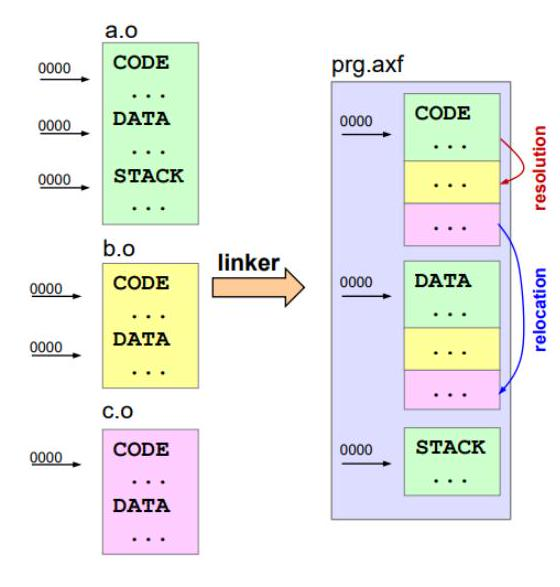
\includegraphics[width=\linewidth]{images/2024_12_29_79e6b22f503fb7b4f718g-10}
\end{concept}

\begin{example2}{Module Interface Example}
\begin{lstlisting}[language=armasm, style=basesmol]
    ; Module A - Defining function
    AREA myCode, CODE, READONLY
    EXPORT myFunction    ; Make available externally
myFunction
    PUSH    {LR}
    ; function code here
    POP     {PC}
    
    ; Module B - Using function
    AREA myCode, CODE, READONLY
    IMPORT myFunction    ; Use external function
    
    BL      myFunction   ; Call the function
\end{lstlisting}
\end{example2}

\begin{KR}{Creating Modular Programs}\\
Steps for modular development:
\begin{enumerate}
  \item Design module structure:
    \begin{itemize}
      \item Identify clear boundaries
      \item Define interfaces
    \end{itemize}
  \item Create individual modules:
    \begin{itemize}
      \item Declare IMPORT/EXPORT
      \item Implement functionality
    \end{itemize}
  \item Compile modules separately
  \item Link modules:
    \begin{itemize}
      \item Resolve references
      \item Create executable
    \end{itemize}
  \item Test integrated system
\end{enumerate}
\end{KR}

\begin{concept}{Guidelines for Modular Programming}\\
Key design principles:
\begin{itemize}
  \item \textbf{High Cohesion}:
    \begin{itemize}
      \item Group related functionality together
      \item Each module fulfills a single defined task
      \item Lean external interface
    \end{itemize}
  \item \textbf{Low Coupling}:
    \begin{itemize}
      \item Minimize dependencies between modules
      \item Clear and minimal interfaces
      \item Easy to modify individual modules
    \end{itemize}
  \item \textbf{Information Hiding}:
    \begin{itemize}
      \item Split interface from implementation
      \item Don't expose unnecessary details
      \item Maintain freedom to change internals
    \end{itemize}
\end{itemize}
\end{concept}

\begin{KR}{Symbol Resolution and Relocation}\\
Steps in linking process:

1. Symbol Resolution:
\begin{lstlisting}[language=armasm, style=base]
    ; In module1.s
    AREA |.text|, CODE, READONLY
    EXPORT func1
func1
    ; function code
    
    ; In module2.s
    AREA |.text|, CODE, READONLY
    IMPORT func1
    BL      func1    ; Reference to resolve
\end{lstlisting}

2. Relocation:
\begin{lstlisting}[language=armasm, style=base]
    ; Before relocation
    BL      func1    ; Relative offset
    
    ; After relocation
    BL      0x08000234  ; Absolute address
\end{lstlisting}
\end{KR}

\begin{formula}{Linkage Types in C}\\
Three types of linkage:
\begin{itemize}
  \item \textbf{External Linkage}:
    \begin{itemize}
      \item Global names available to all modules
      \item Default for functions and global variables
      \item Example:
\begin{lstlisting}[language=C, style=base]
int global_var;           // External linkage
void global_func(void);   // External linkage
\end{lstlisting}
    \end{itemize}
  \item \textbf{Internal Linkage}:
    \begin{itemize}
      \item Names only available within module
      \item Created using 'static' keyword
      \item Example:
\begin{lstlisting}[language=C, style=base]
static int module_var;    // Internal linkage
static void local_func(void); // Internal linkage
\end{lstlisting}
    \end{itemize}
  \item \textbf{No Linkage}:
    \begin{itemize}
      \item Local variables and function parameters
      \item Scope limited to block
      \item Example:
\begin{lstlisting}[language=C, style=base]
void func(void) {
    int local_var;       // No linkage
    static int static_var; // Internal linkage
}
\end{lstlisting}
    \end{itemize}
\end{itemize}
\end{formula}

\begin{example2}{Object File Structure}
Example of complete object file:
\begin{lstlisting}[style=base]
File sections:
1. '.text' section (Code):
0x00000000: 4604  MOV     r4,r0
0x00000002: 0040  LSLS    r0,r0,#1
0x00000004: 4420  ADD     r0,r4

2. '.data' section:
0x00000000: Initial values for global data

3. Symbol table:
#  Name      Value    Type   Binding
6  myFunc    0x0000  CODE   Global
7  extVar    0x0000  DATA   Reference

4. Relocation entries:
Offset   Type         Symbol
0x0006   R_ARM_REL32  extVar
\end{lstlisting}
\end{example2}

\begin{KR}{Library Creation and Use}\\
Steps for creating and using libraries:

1. Create library source files:
\begin{lstlisting}[language=C, style=base]
// lib.h
void lib_func(int x);

// lib.c
void lib_func(int x) {
    // Implementation
}
\end{lstlisting}

2. Compile to object files:
\begin{lstlisting}[style=base]
armcc -c lib.c -o lib.o
\end{lstlisting}

3. Create static library:
\begin{lstlisting}[style=base]
armar --create libmy.a lib.o
\end{lstlisting}

4. Link with library:
\begin{lstlisting}[style=base]
armlink main.o libmy.a -o program.axf
\end{lstlisting}
\end{KR}

\begin{concept}{Tool Chain Components}\\
Essential tools for development:
\begin{itemize}
  \item \textbf{Compiler (armcc)}:
    \begin{itemize}
      \item Translates C to assembly
      \item Performs optimizations
      \item Generates object files
    \end{itemize}
  \item \textbf{Assembler (armasm)}:
    \begin{itemize}
      \item Processes assembly code
      \item Creates object files
      \item Handles directives
    \end{itemize}
  \item \textbf{Linker (armlink)}:
    \begin{itemize}
      \item Combines object files
      \item Resolves references
      \item Creates executable
    \end{itemize}
  \item \textbf{Library Manager (armar)}:
    \begin{itemize}
      \item Creates/maintains libraries
      \item Adds/removes object files
      \item Archives multiple objects
    \end{itemize}
\end{itemize}
\end{concept}

\begin{remark}
Important considerations:
\begin{itemize}
  \item Use consistent naming conventions
  \item Document module interfaces clearly
  \item Consider initialization dependencies
  \item Test modules independently
  \item Maintain version control
  \item Document build requirements
\end{itemize}
\end{remark}